\documentclass[12pt,a4paper]{article}
\usepackage[utf8]{inputenc}
\usepackage[german]{babel}
\usepackage[T1]{fontenc}
\usepackage{amsmath}
\usepackage{amsfonts}
\usepackage{amssymb}
\usepackage{graphicx}
\usepackage[left=2.5cm,right=2.5cm,top=2cm,bottom=2cm]{geometry}
\usepackage{float}
\author{Gruppe C14 \\ Julián Häck, Martin Koytek, Lars Wenning, Erik Zimmermann}

\begin{document}
\section{Bestimmung der Materialeigenschaften der Saiten}
\subsection{Versuchsbeschreibung}
Für den Grundton $f$ einer Gitarrensaite gilt:
\begin{equation}
f=\frac{1}{2}\sqrt{\frac{T}{\mu}}\cdot \frac{1}{l}
\label{Grundgleichung Gitarre f gegen l}
\end{equation}
mit der Saitenspannung T in N, dem Massebelag $\mu$ in $\frac{kg}{m}$ und der Länge der Saite $l$ in m.
In diesem Versuch wird dieselbe Saite bei unterschiedlichen Längen angeschlagen und die entsprechende Frequenz gemessen. Trägt man dann $f$ gegen $\frac{1}{l}$ auf erhält man aus der Steigung $m=\frac{1}{2}\sqrt{\frac{T}{\mu}}$ einen Wert für das Verhältnis von $T$ und $\mu$, das mit den Herstellerangaben verglichen werden sollte.\newline Wir haben uns hier auf die Vermessung der Materialeigenschaften der A-Saite beschränkt.

\subsection{Versuchsaufbau und Durchführung}
\begin{figure}[H]
\centering
\includegraphics[scale=0.1]{Bilder/IMG_20160323_123920.jpg}
\caption{Versuchsaufbau zur Vermessung der Materialeigenschaften der Gitarre}
\end{figure}
Zur Vermessung der Frequenz bei unterschiedlichen Längen wurde die A-Saite zuerst leer, dann im 2ten, 4ten, 6ten, 8ten und 10ten Bund jeweils 3 mal angeschlagen. Die Messung mit Mikrofon und Cassy selbst erfolgte wie im Teilversuch zuvor.
Die Frequenzen selbst wurden mittels Fast-Fourier-Transformation und Peakschwerpunktsberechnung bestimmt. Die jeweils drei Frequenzen wurden dann gemittelt und über Gleichung (\ref{sigmean}) der Fehler auf den Mittelwert bestimmt.
\newline
Die Länge der Anschlagpunkte wurden mit dem Maßband vermessen.\newline

\begin{table}[H]\centering
\caption{Messwerterfassungseinstellungen}
\begin{tabular}{c|c}
Parameter & Einstellung \\ 
\hline
Messintervall & 500 $\mu$s \\ 
Anzahl Messwerte & 10000 \\ 
Messdauer & 5s \\ 
Trigger & 0.3V \\ 
\end{tabular} 
\end{table}

\subsection{Versuchsauswertung}

\subsubsection{Rohdaten}
\begin{table}[H]\centering
\caption{Längenmessungen der Anschlagpunkte}
\begin{tabular}{c|c|c}
$L_0$ & 64.9 cm & Leere Saite\\ 
$L_1$ & 54.6 cm & 2. Bund \\ 
$L_2$ & 51.5 cm & 4. Bund \\ 
$L_3$ & 45.9 cm & 6. Bund \\ 
$L_4$ & 40.9 cm & 8. Bund \\ 
$L_5$ & 36.4 cm & 10. Bund \\ 
\end{tabular} 
\end{table}
Die Messung am 2. Bund wurde in der Auswertung ausgelassen, da die Längenmessung offenbar fehlgeschlagen ist. Die Abstände vom Steg zu den jeweiligen Bünden wurden mit dem Maßband bestimmt, daher haben wir den Fehler auf:
\begin{equation*}
\sigma_L=1 mm
\end{equation*}
abgeschätzt.


\begin{table}[H]\centering
\caption{Frequenzmessung bei unterschiedlichen Längen}
\begin{tabular}{c|cccccc}
 & $L_0$ & $L_1$ & $L_2$ & $L_3$ & $L_4$ & $L_5$ \\ 
\hline 
$f_1$ & 110.16 & 123.80 & 138.98 & 156.03 & 174.60 & 194.42 \\ 
$f_2$ & 110.20 & 123.79 & 139.04 & 155.69 & 174.31 & 196.00 \\ 
$f_3$ & 110.24 & 123.79 & 138.83 & 155.96 & 174.46 & 195.97 \\ 
$\bar{f}$ & 110.20 & 123.79 & 138.95 & 155.89 & 174.46 & 195.46 \\ 
$\sigma_{\bar{f}}$ & 0.02 & 0.00 & 0.06  & 0.10 & 0.08  & 0.52  \\ 
\end{tabular}
\newline 
Angaben in Hz
\end{table}
$~$\newline
Der Fehler auf die Frequenz ist bei der Vermessung des 2. Bunds sehr klein (ungerundet: $\sigma_{\bar{f_1}}=0.0033$). Dieser Wert wurde aber schon wegen der Längenmessung weggelassen.
$~$\newline
$~$\newline
Für die von uns vermessene A-Saite gilt laut Skript:
\begin{equation*}
\mu_{lit}=3.4095 \cdot 10^{-3} \frac{kg}{m}, \hspace{1cm}
T_{lit}=68.04 N.
\end{equation*}
Für die Steigung ist also ein Wert von
\begin{equation}
m_{lit}=\frac{1}{2}\sqrt{\frac{T_{lit}}{\mu_{lit}}}=70.633 \frac{m}{s}
\label{Herstellerangabe Gitarre}
\end{equation}
zu erwarten.
\subsubsection{Transformation der Rohdaten}
Die nun bestimmten gemittelten Frequenzen können jetzt mit ihren Fehlern gegen die jeweiligen Längen mit ihren Fehlern aufgetragen werden.
\begin{figure}[H]\centering
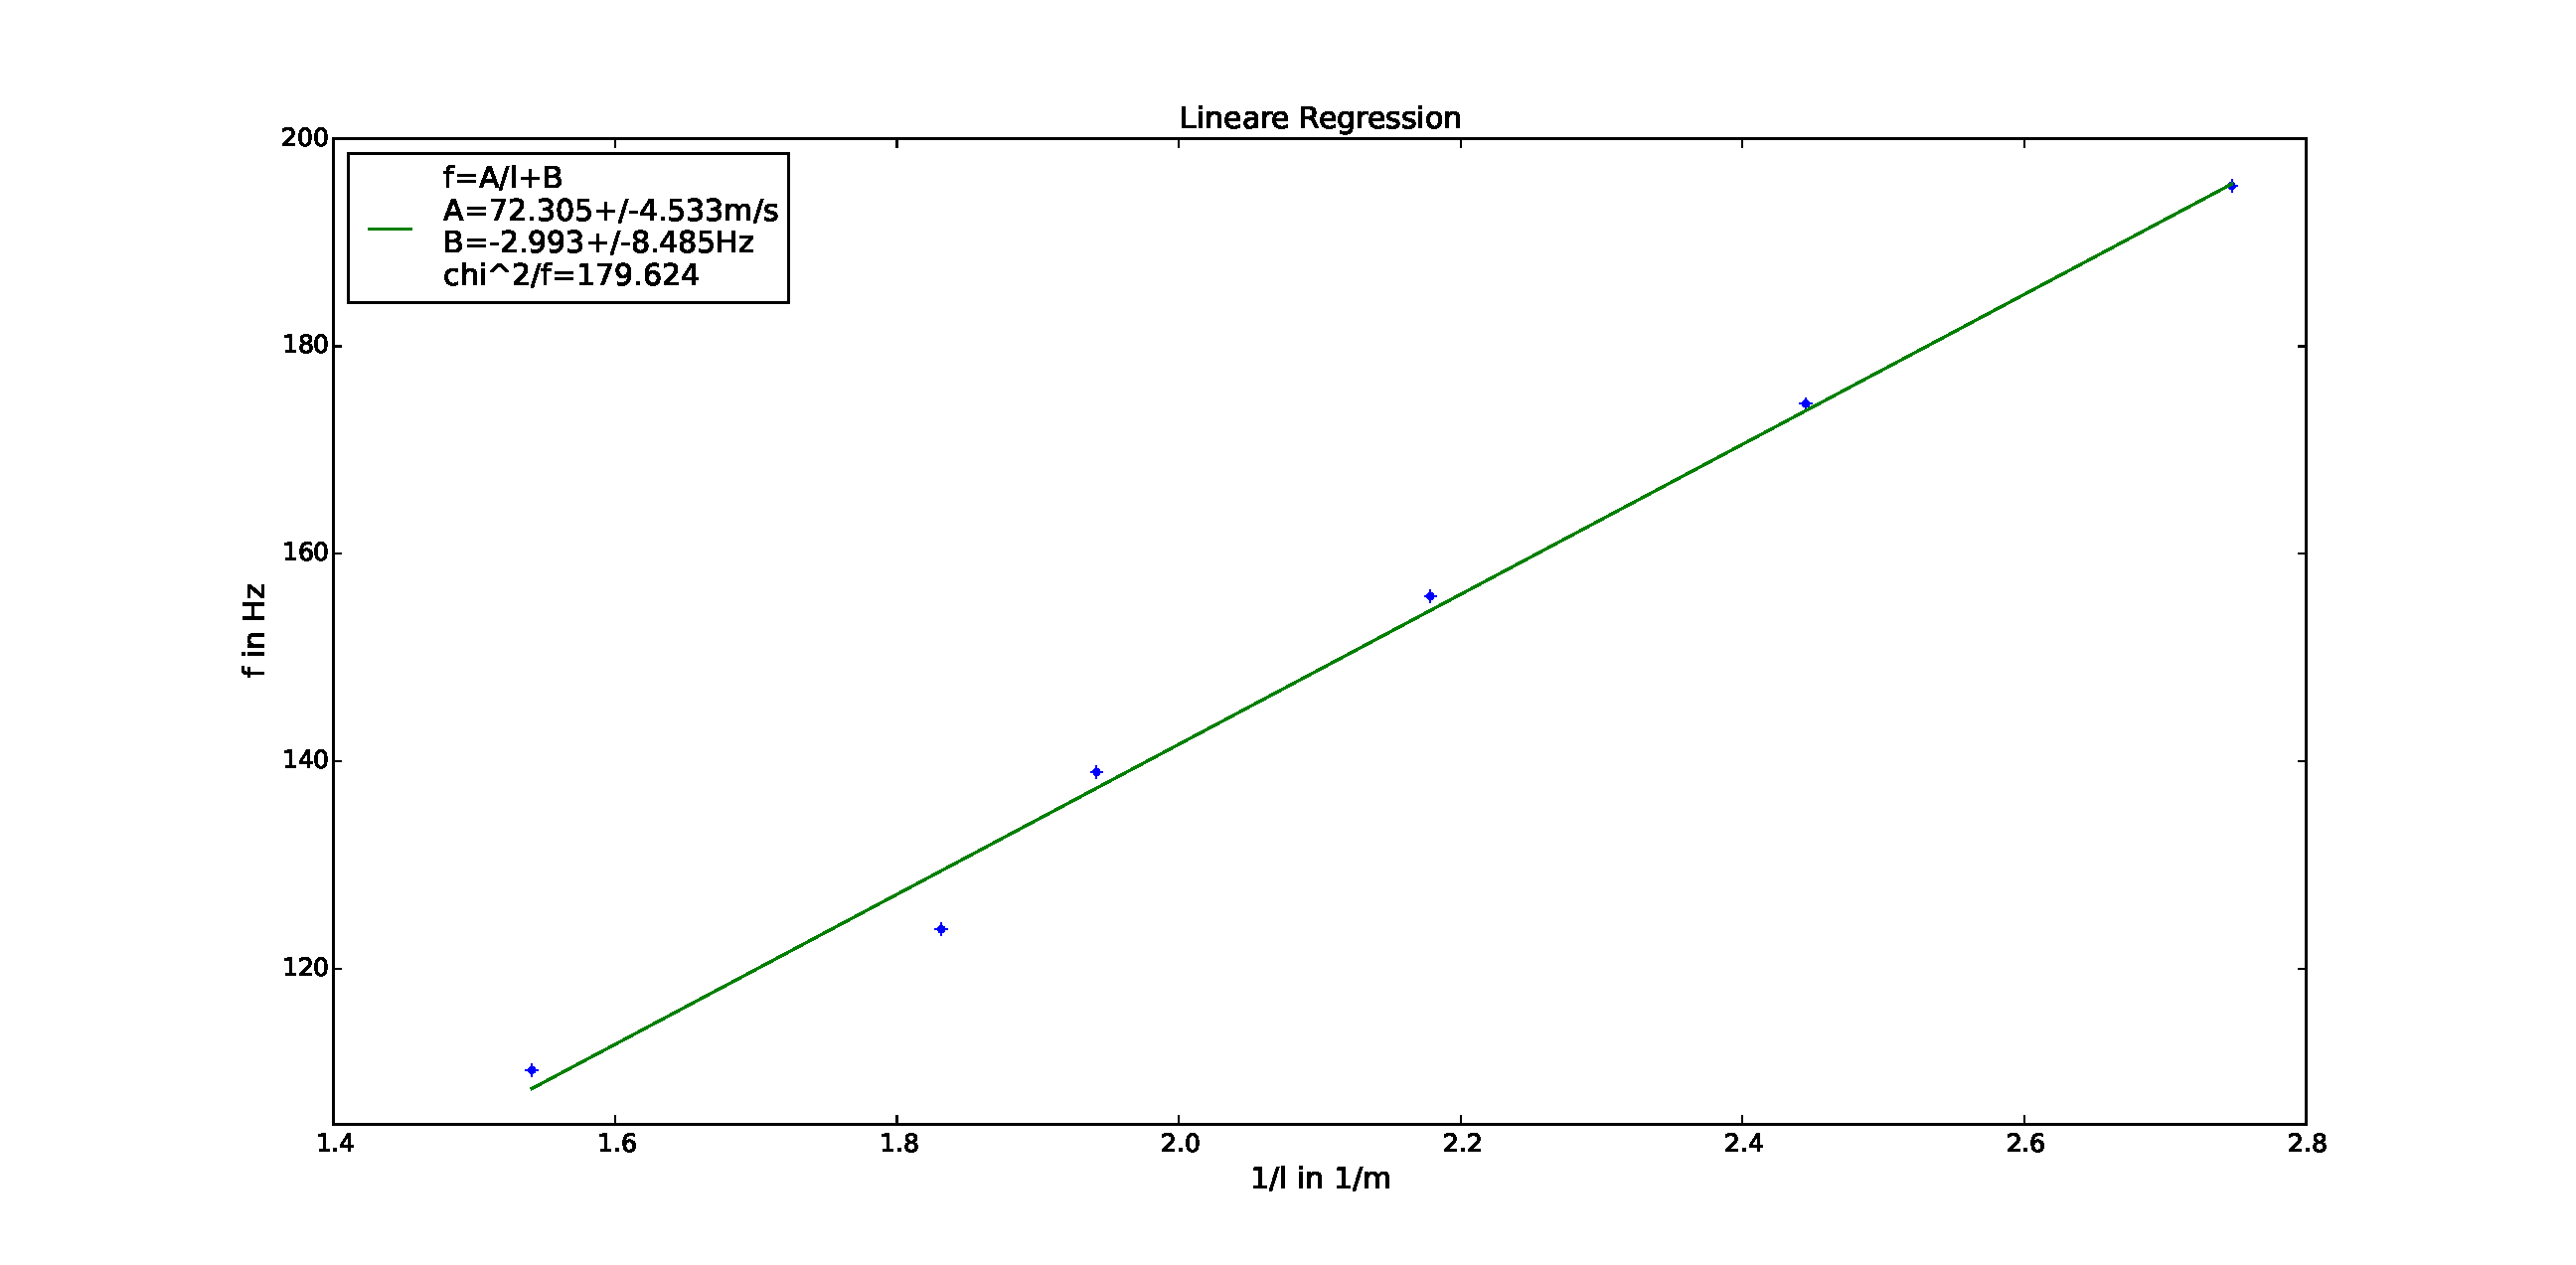
\includegraphics[scale=0.4]{Bilder/lin_reg_mit.eps}
\caption{Lineare Regression aller Werte. Der 2. Wert ist ein deutlicher Ausreißer und wurde daher im Folgenden weggelassen.}
\end{figure}

\begin{figure}[H]
\centering
\includegraphics[scale=0.4]{Bilder/lin_reg_ohne.eps}
\caption{Lineare Regression ohne den zweiten Wert. Der Fehler steigt mit $\frac{1}{l}$, da die Saite bei kürzerer Länge stärker gedämpft ist und nicht so lange schwingt.}
\end{figure}


\begin{figure}[H]
\centering
\includegraphics[scale=0.4]{Bilder/lin_reg_ohne_residuum.eps}
\caption{Residuenplot ohne den zweiten Wert. Der Residuenplot zeigt keine Systematik und alle Messwerte schneiden mit ihren Fehlern die Null-Linie.}
\end{figure}

Ergebnis der Linearen Regression:
\begin{align*}
A = m &= 71.162 \pm 0.282 \frac{m}{s}  \\
B &= 0.612 \pm 0.523 Hz \\
\frac{\chi^2}{f}&=0.601
\end{align*}

Zum Vergleich (siehe Gleichung \ref{Herstellerangabe Gitarre}):
\begin{equation}
m_{lit}=70.633 \frac{m}{s}
\end{equation}

\subsubsection{Fazit}
Der Wert aus den Herstellerangaben liegt im Bereich von 2 Standardabweichungen unter dem gemessenen Wert. Dies ist darauf zurückzuführen, dass die Gitarre im Laufe der Zeit abgenutzt wurde und daher der Massebelag mittlerweile eher kleiner ist als bei der Herstellerangabe für die neue Saite. \newline
Der gemessene y-Achsenabschnitt von $B = 0.612 \pm 0.523$ Hz liegt mit seinem Fehler nahe genug an dem erwarteten Wert von 0 (siehe Gleichung \ref{Grundgleichung Gitarre f gegen l}).
\newline
Das $\frac{\chi^2}{f}$ von 0.601 lässt zwar auf einen leicht überschätzten Fehler schließen, ist aber noch in einem vertretbaren Bereich.

\end{document}